%%%%%%%%%%%%%%%%%%%%%%%%%%%%%%%%%%%%%%%%%%%%%%%%%%%%%%%%%%%%%%%%%%%
%
% IMPERIAL COLLEGE LONDON DISSERTATION TEMPLATE 
%
%%%%%%%%%%%%%%%%%%%%%%%%%%%%%%%%%%%%%%%%%%%%%%%%%%%%%%%%%%%%%%%%%%%
%
% Copyright (c) 2008, Daniel Wagner, www.PrettyPrinting.net
% http://www.prettyprinting.net/imperial/
%%%%%%%%%%%%%%%%%%%%%%%%%%%%%%%%%%%%%%%%%%%%%%%%%%%%%%%%%%%%%%%%%%%

\documentclass[MSc,paper=a4,pagesize=auto]{icldt}
%\usepackage{showframe}
%\usepackage{cleveref} % lets us use chapter references
\usepackage{graphicx}  % lets us import graphics nicely
\usepackage{subcaption}  % lets us use subfigure
\usepackage[binary-units=true]{siunitx}   % and friendly SI unit shiz
\setcounter{tocdepth}{1} % don't show sub-sections in the TOC

% next two lines supress 'underfull hbox" warnings caused by URLs in bib file
\usepackage{etoolbox}
\apptocmd{\sloppy}{\hbadness 10000\relax}{}{} 

% Essential Setup
\title{Seeing the Big Data: Virtual Reality Visualisations of Large Datasets}
\author{Alexander Zawadzki (az2713)}
\date{September 2014}
\department{Computing}

% Optional
\supervisor{Professor Daniel Rueckert} 
\dedication{
My thanks to: 
\newline
\newline
Dr Paul Gass and Dr Ian Thompson, my bosses at Sharp Laboratories of Europe Ltd., for arranging for my funded sabbatical year at Imperial College London. 
\newline
\newline
Colleagues 	Dr Nathan Smith, Dr Graham Jones, Dr Jon Mather, and Dr Andrew Kay for sharing their passion for 3D display systems. Especial thanks to John Nonweiler, for setting an example of how development software \textit{should} be done.
\newline
\newline
Supporters Aashish Chaudhary at Kitware, and Brad Davis at ORIA for providing insight into VTK and the Oculus Rift SDK respectively.
\newline\
\newline
Friends in the MCS Program, in particular coffee-break-buddies Moritz Schrenk and Tereza Drskova. 
\newline
\newline
And last, but not least, I am indebted to my supervisors Professor Daniel Ruckert and Dr Bernhard Kainz. You have provided freedom when I wanted it, and guidance when I needed it. I am deeply grateful to you both. 
}

\begin{document}
\maketitle

\begin{abstract}
%\textbf{A Zawadzki, Department of Computing, Imperial College London}
%\\ \textbf{Abstract of Master's Thesis, submitted September 4th 2014}
%\\ \textbf{Seeing the Big Data: Virtual Reality Visualisations of Large Datasets}
A new pipeline is implemented for the visualisation of Human Connectome Project (HCP) data. HCP data are converted to an intermediate format, and then imported into the Visualisation Tool Kit (VTK). Through a series of extensions to the VTK pipeline, the data are rendered as distorted stereographic 3D images and output to an Oculus Rift virtual reality headset. Sensors on the headset track the user's head position and dynamically update the rendered image. The complete pipeline allows an immersive 3D display of data, with native access to all VTK functionality. A user study is conducted to evaluate the pipeline, and the resulting strengths and weaknesses are discussed.

%\hfill --- Alexander Zawadzki

\end{abstract}

\makededication
%\iffalse
\tableofcontents

\listoftables
\listoffigures


\chapter{Introduction}
\section{Context}
In order to better understand the functioning of the human brain, the neurology of the brain is very important. The Human Connectome Project (in the USA) and the Developing Human Connectome Project (in the UK) are ongoing projects dedicated to mapping and analysing the neural connections of developed and developing human brains. 

The Connectome projects produce very large datasets giving information about the structural or functional connectivity of neurons in the brain. The volume of data produced, and 3D nature of the data makes it difficult to visualise in a 2D form. A typical functional connectome matrix, for example, may have 3,000 by 3,000 elements and in 2D form bears no resemblance to the physical shape of the fibres.

This project aims to develop new visualisation techniques for looking at connectivity data in 3D by using commercial virtual reality tools. Specifically, the Oculus Rift will be used to display a 3D model of the brain, over which connectome data can be superimposed. This approach should be equally applicable to visualising structural and functional connectivity. 

<TODO: Use elements of the following...>

The growth of computing power and the volume of data available for analysis has far outpaced the development of visualisation hardware. In medical imaging multi-gigabyte datasets are common: as of June 2014 the Human Connectome Project has generated over 20 terrabytes of data on the three dimensional structure of the human brain. Courtesy of Moore's Law, the hardware available to process these data sets is growing exponentially. Display hardware has been constantly evolving. Unwieldy cathode-ray-tubes have morphed into slim LCSs less than one millimetre thick. Touch-screens became ubiquitous and tablet computers became commonplace. All of the dominant technologies share a common feature - they display 2D information for a user to look at. This situation may be set to change. 

Recent developments in virtual reality hardware offer a  paradigm shift in display technology. The change may see the popularity of displays that overlay information on top of the real world, so-called 'augmented reality', or displays that can provide a completely artificial 'virtual reality' experience. In either case, the displays will provide an immersive, three dimensional experience quite unlike any established technology today.

It is exhilarating and sometimes intimidating to be at the forefront of such a dynamic field. Since the project was initially planned, Oculus have significantly re-designed their Software Development Kit three times. In response to this, the ORIA project fundamentally revised their their book before it was even published. VTK continues to be developed and released on a daily basis, adding (and sometimes removing!) important features.

\newpage
\section{Contributions}
This project has investigated the use of consumer grade virtual reality hardware, specifically the Oculus Rift DK1, as a tool for visualising and interacting with large datasets. The project has contributed to the open source community in a number of ways:

\begin{itemize}
  \item A plug-in was developed for Blender in order to allow the import of legacy .vtk format data.
  \item The excellent Oculus Rift in Action (ORIA) project was forked on GitHub, at the suggestion of the project owner Brad Davis, to share bug-fixes with the community.
  \item Source code was ported from Paraview with encouragement from lead developer Aashish Chaudhary in order to bring Rift functionality to VTK.
  \item When relevant, assorted software problems were documented on Stack Overflow in 'Question and Answer' format. The response to these posts has been very positive, bumping my account "\textit{GnomeDePlume}" to the top quartile of contributors in 2014.  
\end{itemize}

In comparison to the size and scope of these established projects, this project has made only incremental contributions. Nevertheless, these contributions have been contributed in the spirit of open source collaboration and have have incrementally advanced the state-of-the-art.

The academic impact of this project is more difficult to quantify. TODO: suggestions welcome! Virtual reality hardware is not widely available, although the sudden success of the Microsoft Kinect has highlighted the explosive adoption of new technology into research when available at commodity prices.

\newpage
\section{Structure of the Report}
As the project dealt with implementing a pipeline, illustrated in Figure~\ref{fig:the_full_pipeline}, it seems natural for the report to follow the process from raw data acquisition to the final display image. 

Following this logic, Chapter~2 discusses the how the Human Connectome Project (HCP) maps human brain structures using DTI and fMRI imaging, and discusses existing visualisation techniques. Chapter~3 discusses the HCP data structure, and how it may be converted to intermediate formats. Chapter~4 shows how a Visualisation Tool Kit (VTK) pipeline can be constructed and HCP data can be processed for interaction and display on a standard 2D computer monitor. 

Chapter~5 breaks away from the sequential structure in order to introduce the Oculus Rift hardware, and shows how the collimating optics in the headset will distort images unless extra distortion shaders are used. The report then returns to the VTK pipeline in Chapter~6 to discuss the good, the bad and the ugly ways to apply shaders so that images can be rendered correctly to the Rift Virtual Reality (VR) headset. 

\begin{figure}[htbp!]
    \centering
    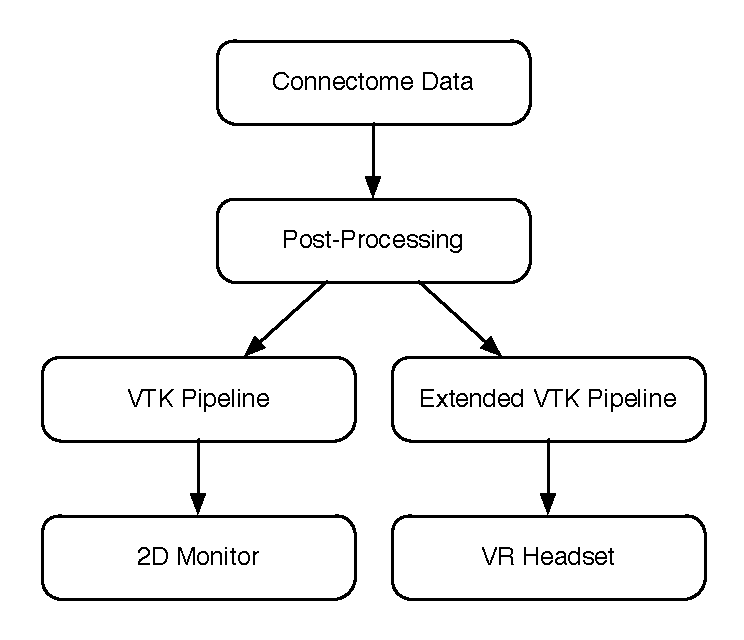
\includegraphics[scale=0.5]{resources/data_pipeline_overview}
    \caption{The Full Pipeline}
    \label{fig:the_full_pipeline}
\end{figure}

With a complete pipeline for VR, Chapter~7 discusses how the system was evaluated. This evaluation identified numerous strengths and weaknesses, and suggestions for further work are explored.

Finally, Chapter~8 concludes by synthesizing findings from each stage in the project, and reviewing the most interesting learning outcomes.

\chapter{Connectome Data}
\section{Motivation for using Connectome Data}
Mapping and visualising the brain is of considerable academic and practical interest. The brain is thought to be composed of motor, sensory, behavioural state, and cognitive systems \cite{Swanson2003}. Better knowledge about the physiology of the brain can help in understanding these systems. Knowledge of the structure of an individual brain can also be very helpful when diagnosing medical conditions, or planning a surgical procedure \cite{Golby2011}. In either case, the interested parties need to have data, and to be able to draw useful inferences from it. This project aims to work on the second of these challenges: to develop new ways of displaying and interacting with existing connectome data. 

\section{Sources of Connectome Data}
An understanding of the processes for generating connectome data is useful, as it influences the resolution and format of the data. The most relevant methods:
\begin{enumerate}
\item Electron microscopy (EM) gives nanometer resolution images of neural structure. This is an ex vivo process, samples must be taken from the brain. EM techniques can give a resolution of \SI{5}{\nm} in the x-y plane, with a \SI{30}{\nm} slice thickness and generate an enormous amount of raw data, of the order of \SI{1}{\pebi\byte\per\mm\cubed} \cite{Jeong2010}.\footnote{That data density is greater than two hundred thousand DVDs per cubic milimeter or, in old money, more than eleven \textit{billion} floppy disks per cubic inch} Due to the high resolution and small sample sizes accommodated by EM techniques, the only connectome to have been completely mapped out by this technique is that of the nematode c.elegans \cite{White1986}.
\item Optical microscopy (OM) techniques can be used in conjunction with fluorescent markers to selectively tag and examine brain matter. As with EM, this is done ex-vivo. This approach allows for much larger samples to be analysed, at a resolution of approximately \SI{0.35}{\um} in the x-y plane, and with a slice thickness of \SI{100}{\um}. This approach has recently been used to map the entire mouse connectome \cite{Oh2014}. 
\item Magnetic Resonance Imaging (MRI) scans may be used in combination with Diffusion Tensor Imaging as an in-vivo technique for determining larger scale structure. Diffusion of water within the brain is influenced by the structure of the brain matter, since water can diffuse more easily along bundles of nerves than perpendicular to them, and so the diffusion patterns allow local structure to be inferred. The resolution of this technique is typically low, approximately \SI{1}{\mm} in the x-y plane \cite{Westin2002}. MRI techniques have been used to map hundreds of human connectomes. 
\end{enumerate}

\section{Storing Connectome Data}
There are no standardised formats for storing connectome data, and the form of raw data depends on the experimental technique used to obtain it (EM, OM, DT-MRI) and the specific equipment used. Many tools such as NeuroneJ \cite{NeuronJ2014}, Imaris \cite{Imaris2014}, and Amia \cite{Amira2014} have been developed for manipulating connectome data, but these tools can require a specific input data format. 

Alternatively, it may be necessary to implement a custom data structure. Fast access to the data is essential when working interactively with high resolution images. Previous publications \cite{Jeong2010} have discussed working with a 75GB connectome dataset, stored as an octree in order to enable fast access to the desired parts of the dataset. They also store sub-sampled data at various resolutions in order to allow responsive zooming into the data set and cache data at GPU, CPU and process levels. 

\section{Visualising Connecome Data}
A number of common visualisations exist for connectome data. Visualisations can be divided into three types: structural, functional and multimodal. Some visualisations, connectivity matrices for example, are equally well suited to display structural or functional information. Other visualisations, such as tractographies, are best suited to displaying structural information. Multimodal visualisations show elements of both structural and functional data. Virtual reality is well suited to display structural information, and so the following visualisations discussed are primarily those for structural or multimodal data.

\subsection{Connectivity Matrix}
A connectivity matrix shows the physical or functional connectivity between different regions of the connectome \cite{Wang2011}. It allows a lot of information to be presented in a single 2D image. However, it does not represent the spatial relationship of the data, and the format in which the axes are ordered may introduce false patterns. 

\begin{figure}[htbp!]
    \centering
    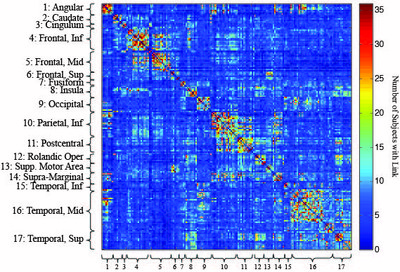
\includegraphics[width=0.5\textwidth]{resources/connectivity_matrix}
    \caption{An alphabetically ordered connectivity matrix. \cite{Wang2011}}
    \label{fig:connectivity_matrix}
\end{figure}

\subsection{Tractography}
Tractography is the process of visualising nerve tracts, bundles of nerve cells. It can provide a very intuitive way of looking at nerve data. It can can require considerable manual editing of opacity, colour and shading in order to bring out the desired features in a tractography image. Without such editing, tractography images suffer from a surfeit of information and can obscure features of interest.

\begin{figure}[htbp!]
    \centering
    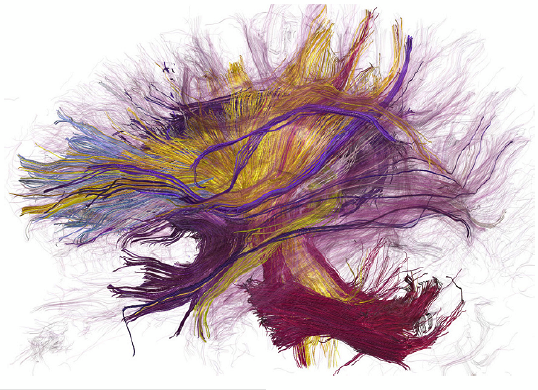
\includegraphics[width=0.8\textwidth]{resources/tractography}
    \caption{Fiber Tractography. \cite{Odonnell2006}}
    \label{fig:tractography}
\end{figure}

Various techniques have been developed for fiber tractography, including the use of tuboids, streamlines and streamtubes to represent the tracts. These techniques can offer a host of advantages including faster rendering times, aesthetically pleasing labelling of tracts, simplified tract junction rendering and good occlusion handling \cite{Petrovic2007}.

\begin{figure}[htbp!]
    \centering
    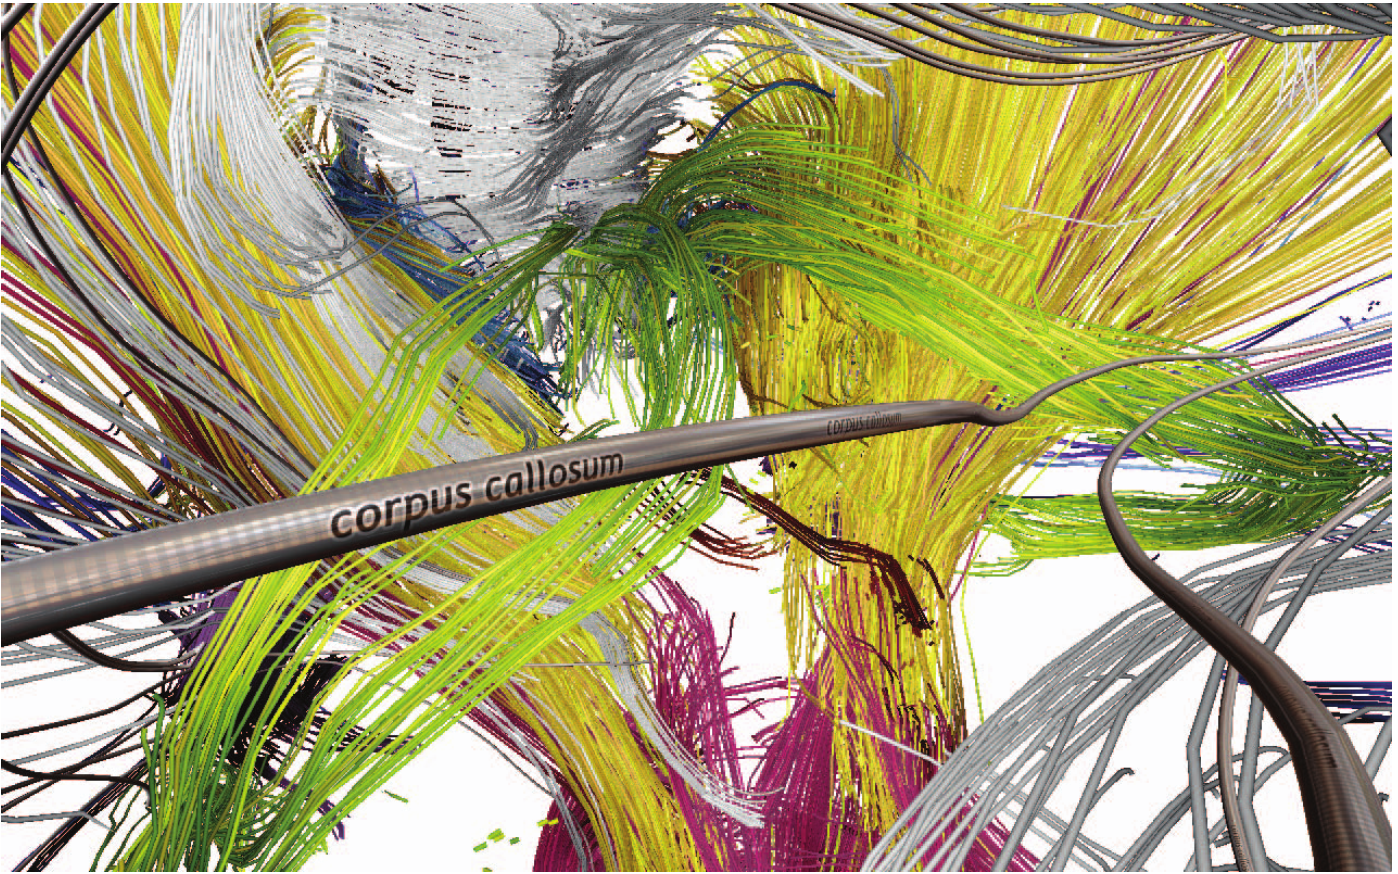
\includegraphics[width=0.8\textwidth]{resources/tuboids}
    \caption{A tractography image using tuboids. \cite{Petrovic2007}}
    \label{fig:tuboids}
\end{figure}

\subsection{Glyph Images}
Glyphs can be used to represent local diffusion tensors in DT-MRI data. The goal of glyph images is to show local diffusion properties as well as larger macroscopic structure. Various systems have been proposed to do this: using ellipsoids \cite{Pierpaoli1996}, colour coded arrows \cite{Peled1998}, opacity mapping \cite{Westin1997}, and hybrid geometric shapes \cite{Westin2002}. 

A spherical glyph represents isotropic diffusion properties, whereas various ellipsoids can represent a local bias towards linear or planar diffusion. Local diffusion can be represented as an ellipsoid or, due to the ambiguity in representing a 3D ellipsoid in a 2D image, as a hybrid shape.

\begin{figure}[htbp!]
    \centering
    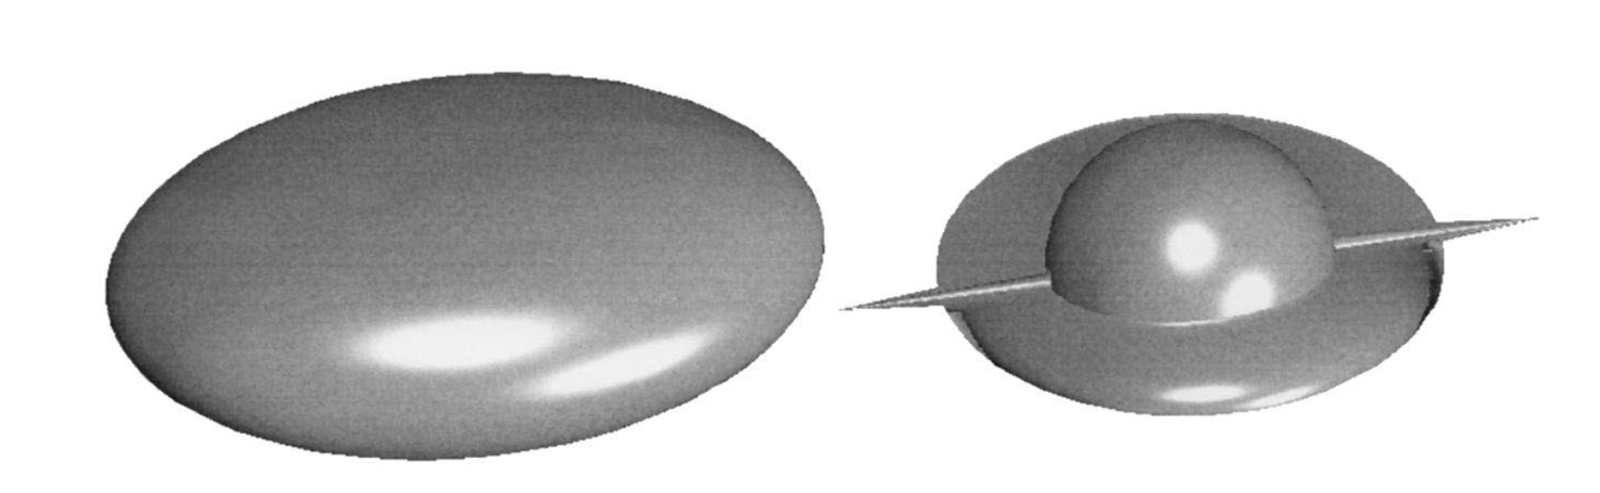
\includegraphics[width=0.6\textwidth]{resources/hybrid_glyphs}
    \caption{Hybrid glyphs representing local diffusivity in DT-MRI data. \cite{Westin2002}}
    \label{fig:hybrid_glyphs}
\end{figure}

The ordered placement of glyphs can introduce patterns not present in the data, prompting research into the positioning of the glyphs, and the use of particle systems to re-position glyphs as a function of interparticle forces \cite{Kindlmann2006}. The benefit of this approach is that the sampling artefacts may be greatly reduced or completely removed from the final image. As can be seen from the figure below, this approach is not without drawbacks, new image artefacts, such at the hexagonal close packing structure, may be introduced by the particle field. 

\begin{figure}[htbp!]
    \centering
    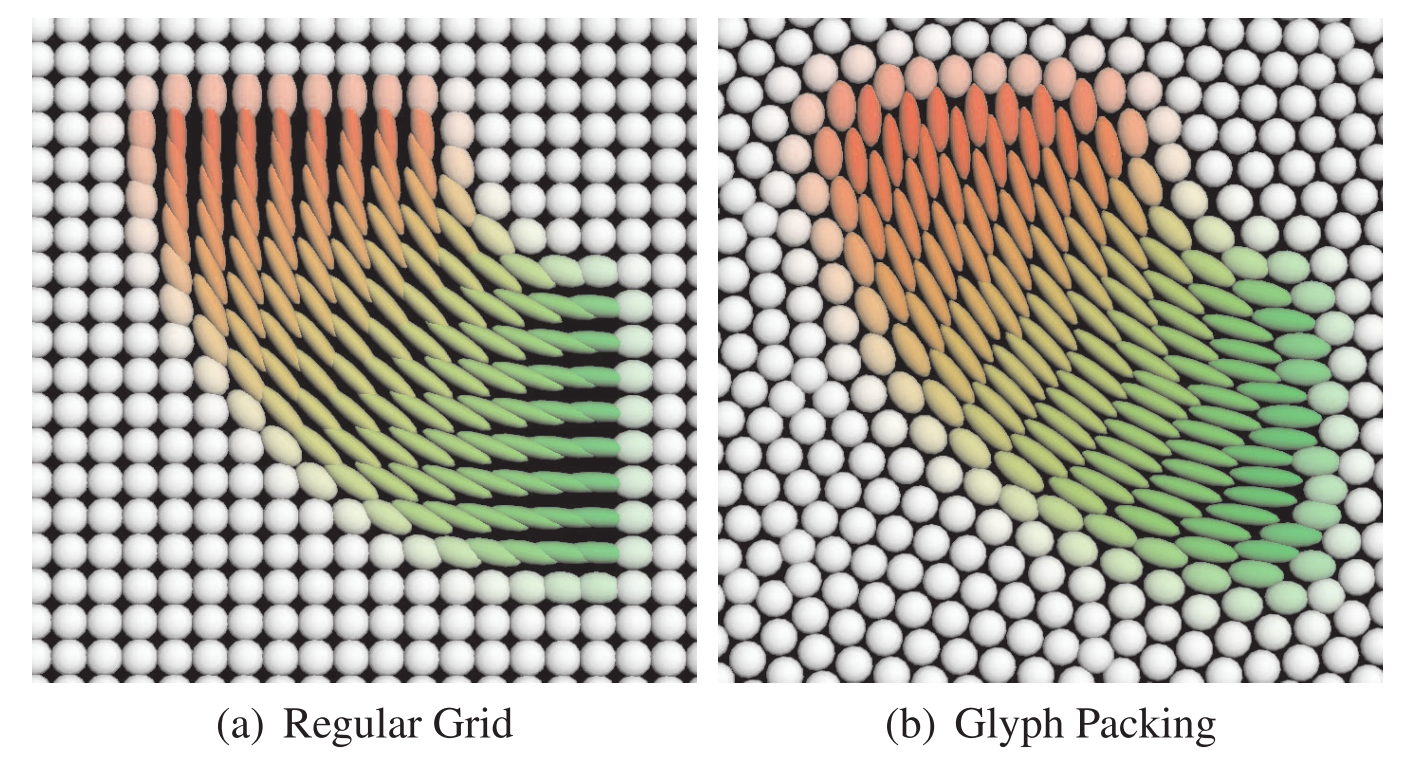
\includegraphics[width=0.6\textwidth]{resources/glyph_packing}
    \caption{Glyph packing. \cite{Kindlmann2006}}
    \label{fig:glyph_packing}
\end{figure}

\subsection{Other Techniques}
In addition to connection matrices, tractographies and glyph images there are a large number of other ways to display connectome data. Graph-based representations can present functional connectivity \cite{Hagmann2008}, but may do so at the cost of reduced anatomical accuracy \cite{Margulies2013}. 

\begin{figure}[htbp!]
    \centering
    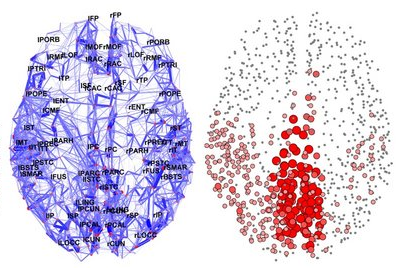
\includegraphics[width=0.8\textwidth]{resources/connectome_graphs}
    \caption{Network structure and interconnection density maps. \cite{Hagmann2005}}
    \label{fig:connectome_graphs}
\end{figure}

The Glass Brain project has developed a multimodal technique for combining structural and functional data \cite{GlassBrain2014}. This type of representation may be useful as it gives anatomical context alongside functional information. 

\begin{figure}[htbp!]
    \centering
    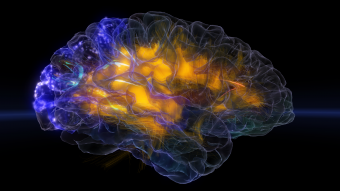
\includegraphics[width=0.8\textwidth]{resources/glass_brain}
    \caption{A Glass Brain visualisation. \cite{GlassBrain2014}}
    \label{fig:glass_brain}
\end{figure}

\section{Summary}
For the purpose of this project, it is useful to note that, with the exception of the connection matrix, all of the visualisation techniques for connectome data attempt to represent 3D (or greater dimensionality) information in a 2D image. This is has two important consequences:
\begin{enumerate}
\item It shows that there is a need to display 3D data.
\item It shows that, in many cases, three dimensional processing and rendering is already being done.
\end{enumerate}

2D representations have a number of advantages. The sampling methods used in measuring the connectome data gather 2D data, the full connectome structure being reconstructed from many planar slices. Relatively little processing is needed in order to convert an array of data into a viewable image, and so a 2D visualisation can be a very fast way to look at raw data. The ‘flat’ nature of 2D images makes them very simple to display or print, to transport and to store. 

Pseudo-3D images are frequently used. These use either colours or symbols to represent out-of-plane structure. Alternatively, they may show a 3D representation of the connectome, rendered into a 2D picture. Using this definition of ‘pseudo-3D’, all of the above visualisation techniques (except the connection matrix) would fall into this category. 

Full 3D images seem very well suited to visualising connectome data. Given that there is a need to display 3D data, and that much of the data is already processed and rendered as a 3D model, it seems natural to displaying it natively in 3D. If the only objections to 3D visualisations is the expense of current 3D hardware \cite{Margulies2013} then a proliferation of cheap consumer hardware may remove this barrier in the near future. 

\chapter{Post-Processing}
Data-wrangling was an important component for this project. The HCP dataset contains a lot of data that is irrelevant to this project, as shown in Figure~\ref{fig:hcp_full_data_set}, so a decision was made to pick a structural example.  The format of that structural data was then awkward: nifti, cifti and gifti aren't perfectly suited for parsing into a graphics program. So a number of alternatives were evaluated for parsing the data. On a pragmatic basis, mitk was used to select a cortical region and export it as an intermediate format (vtk) which is beautifully simple and contains structural information in plain text (hooray!). An import plugin was written for Blender in order to allow this data to be imported and cleaned with some of Blender's excellent mesh manipulation tools. The chapter concludes with the data in a suitable format for VTK input. The (optional) ability to run data through Blender is a bonus, but not necessary for the pipeline.

\section{The Structure of HCP Data}
The HCP data is intended to be a standard format, allowing for comparison between hundreds, eventually thousands, of individual human connectomes. Chapter 2 discussed the different types of experimental data used to measure the connectome structure, and this knowledge quickly helps narrow down the search space. Figure~\ref{fig:hcp_full_data_set} shows that the small fraction of the HCP data set: minimally processed MRI data.  

\begin{figure}[htbp!]
    \centering
    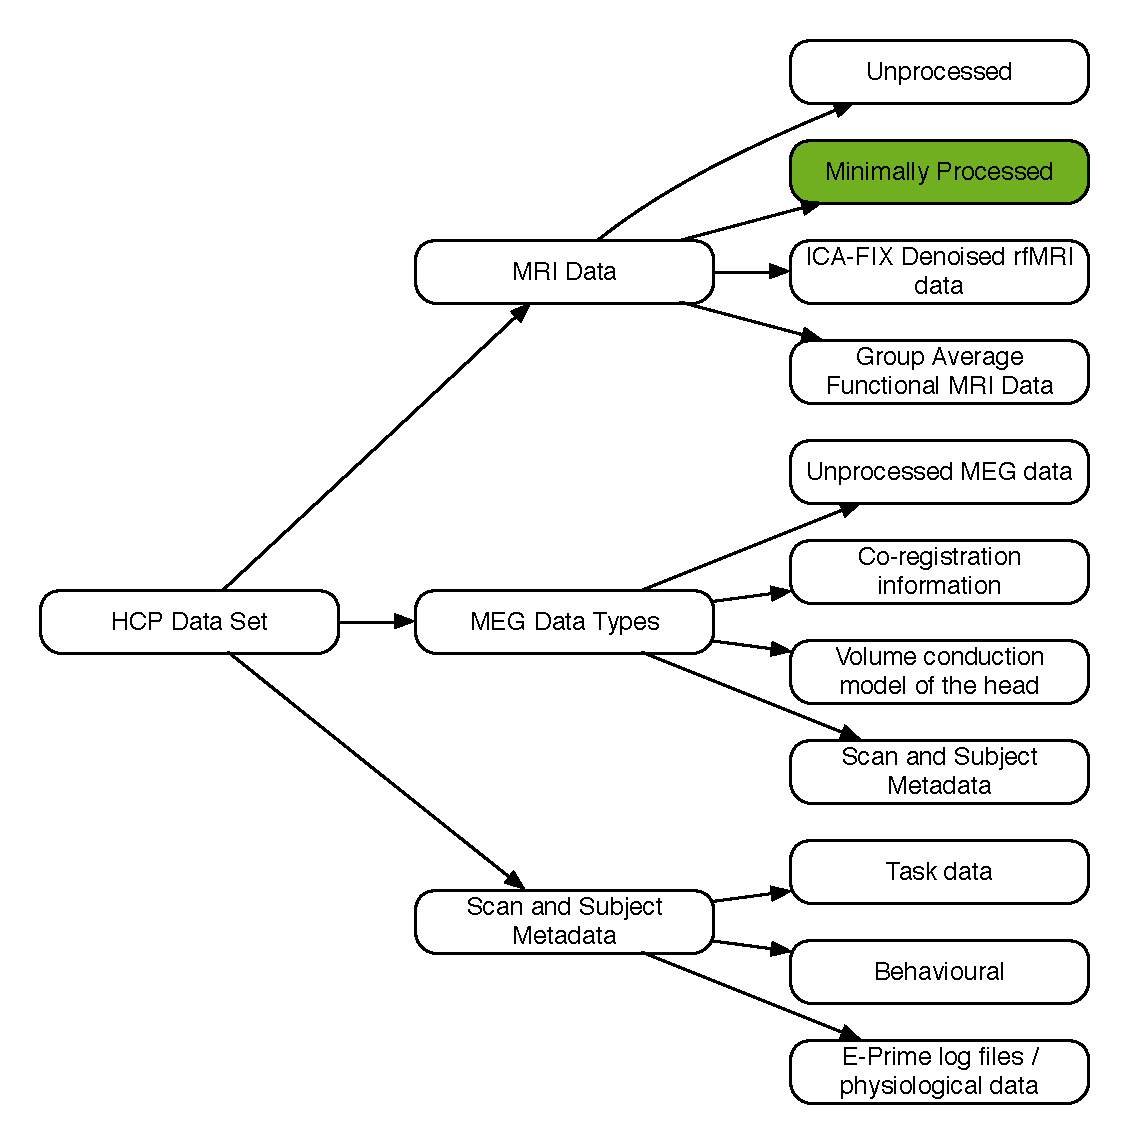
\includegraphics[width=0.8\textwidth]{resources/hcp_full_data_set}
    \caption{Components of a sample HCP Data Set.}
    \label{fig:hcp_full_data_set}
\end{figure}

\section{Choosing an Intermediate Format}

\section{Importing Data to Blender}

\section{Mesh Analysis and Simplification}

\chapter{The Visualisation Tool Kit}
This chapter introduces the Visualisation Tool Kit (VTK), explaining why VTK is an appropriate tool for the project. A simple VTK rendering pipeline is then described, to provide context for subsequent developments. The simple pipeline is modified to work with real connectome data, and additional manipulation tools are added. Finally, the pipeline is modified so that it can produce stereoscopic image pairs.

\section{Introducing VTK}
VTK is a software system for 3D computer graphics, image processing, and visualisation. For the purpose of this project, it's defining characteristics are:
\begin{enumerate}
\item \textbf{It is an open source project, freely available via GitHub.} This proved to be very useful, as the software could be cloned and built immediately and without needing to pay any license fees. The C++ source code was a useful supplement to documentation and tutorials, since it allowed the source to be searched or 'grep-ed' and read. Access to the source code proved to essential when the project needed to extend VTK functionality via subclassing. 
\item \textbf{It is mainly written in C++.} This was useful at a practical level, as the MSc course had provided an introduction to C++. The development model of VTK is to provide core functionality in C++ and then support other languages such as Java and Python using wrappers. This model meant that any functionality added to VTK during this project could be extended to other languages through automatically generated wrapper code.
\item \textbf{It is under active development, and used extensively by the medical imaging community.} The active development of VTK was useful as it meant that there was a substantial volume of documentation and forum material surrounding the software. This meant that it was often possible to learn from past examples and avoid well known problems. The development of VTK by the medical imaging community also meant that VTK could work with medical data formats (well... sort of. Only in 6.x, which I couldn't use) and that there was a known user group who would be interested in any useful developments.
\item 
\end{enumerate}

Developed by Kitware Inc., VTK works well with CMake, and can run on all of the major OS platforms. VTK is also used to do all of the Visualisation work inside Paraview, as well as other notable open-source projects including 3DSlicer.

\section{The VTK Pipeline}
The VTK pipeline is illustrated in Figure~\ref{fig:vtk_pipeline}, with a VTK cone primitive in place of more complex data. In order to use connectome data, it is necessary to load the data as a source. The source must be in a format the VTK can then map to primitives, which places a restriction on the nature of the input data.

Some important components are hidden in this basic pipeline: neither the light nor the camera in the render scene are	 shown. These are both contained in the Renderer, and if not explicitly set then VTK initializes them to default values. This behaviour is simultaneously a great strength and a great liability: it allows a rendering pipeline to be set up very quickly, but it does require that the user be familiar with the pipeline and the various default settings.

\begin{figure}[htbp!]
    \centering
    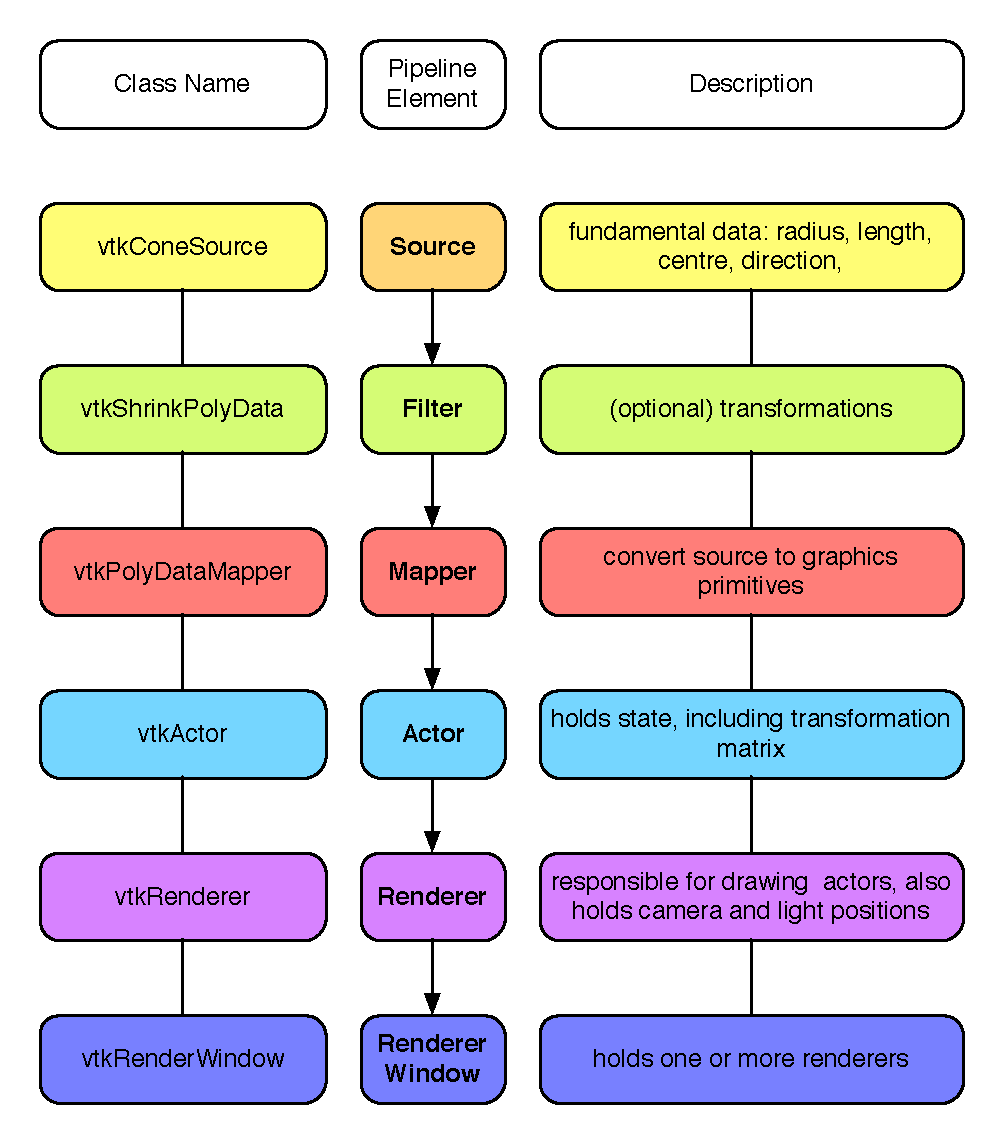
\includegraphics[width=1\textwidth]{resources/vtk_pipeline}
    \caption{The Basic VTK Pipeline for a Cone Primitive}
    \label{fig:vtk_pipeline}
\end{figure}


\section{Complex Data Sources}
Loading and rendering connectome data can be relatively straightforward. Compatibility with a wide range of input data formats was one of the reasons why VTK was chosen as the tool kit to use for the project.

\begin{figure}[htbp!]
\centering
\begin{subfigure}{0.5\textwidth}
    \centering
    
\includegraphics[width=0.4\linewidth]{resources/placeholder}
    \caption{Cone}
	\label{fig:sub1}
\end{subfigure}%
\centering
\begin{subfigure}{0.5\textwidth}
    \centering
    
\includegraphics[width=0.4\linewidth]{resources/placeholder}
    \caption{Cortical Surface}
	\label{fig:sub2}
\end{subfigure}    
    \caption{HCP Data Rendered Using VTK}
    \label{fig:data_sources}
\end{figure}


VTK can read in a large number of file formats including NIfTI (.nii) and VTK's own '.vtk' extension. During testing, a cortical surface data set was used, stored as a \SI{107}{\mebi\byte} '.vtk' file. This was easily read with a vtkReader object and mapped in as polydata. The impact of the large file size, or more accurately the complexity of the object to render, on rendering speed should not have been sufficient to cause visible latency.

\section{Interaction and Callbacks}
Rendering a scene in a continuous loop is a very computationally inefficient technique. It is much better to only re-render the scene in response to a trigger such as a keypress or mouse movement event. Mouse movement is such a common interaction style that it is implemented in VTK using the vtkInteractor object, and even comes with a number of default styles including 'trackball' and 'joystick' modes. Responding to key presses was implemented using a listener  / callback paradigm. VTK conveniently deals with all aspects of logging and queuing the key press, and can trigger a function in response to the event. 

A virtual reality system is a little more demanding than a normal 2D interface since the viewpoint may be continuously moving as the user's head changes position. Ideally the scene would be re-rendered in response to very small changes in head position. The sensors in the HMD report the head position in floating point units, and the precision is so high that any two position queries show some difference. It would be trivial to set thresholds for the pitch, roll, and yaw that would trigger a re-render of the viewpoint but this solution contains it's own problems. Most significantly, if a \SI{5}{\degree} change in head pitch is required to trigger a re-render of the scene, then the scene is always going to jump a minimum of \SI{5}{\degree} in response to changing head position. An attractive alternative solution is to use a clock timer in order to re-render at a fixed frame rate, irrespective of the user's head position. If the system can cope with rendering imagery at \SI{60}{\Hz} then a \SI{16}{\ms} timer should result in smooth scene movements independent of the user's movements.

Interaction for a naive stereo system holds one additional terror. VTK's automatic mouse interactors operate per-renderer, but a the stereo cameras need to be updated simultaneously to prevent the user going cross-eyed. Fortunately, VTK provide a snippet of Python code illustrating how to work around this restriction. The trick is to ensure that the active mouse interaction affects all cameras in the scene, using temporary variables to store each interactor id. 

\section{Rendering Stereo Images}
Rendering stereo images is beautifully intuitive. Stereoscopic 3D involves viewing different images with each eye in order to get an impression of depth. Using VTK, it is possible to create two cameras and position them as if they were eyes viewing objects in the scene. For comfort, the images should be generated using a camera spacing similar to that of the user's Inter-Pupillary Distance (IPD)\footnote{for most of the population this can be safely approximated as \SI{62}{\mm}} although nearby objects in a scene can cause discomfort even when the camera separation is set correctly. The reason for this is that the human visual system copes badly with extreme vergence - it is difficult to focus on an object very close between the eyes\footnote{and for exactly the same reason it is uncomfortable when 3D movies insist on bringing things too close to the audience!}. 

VTK does contain a 'stereo camera' class, but the documentation for this is rare, and implementation usually involves colour anaglyph or interlaced stereographic image systems. The rift needs stereo input to be available in a 'side-by-side' format, and the most basic method of implementing this was to use two separate renderers, each of which was associated with an independent monoscopic camera 

\chapter{Displaying Images on the Rift DK1}
\section{An Introduction to Virtual Reality}
Virtual Reality (VR) refers to the visualisation of an artificial environment. This distinguishes it from Augmented Reality (AR) where the user simultaneously experiences real and virtual environments. The Oculus Rift is a VR device since it completely shuts out any view of the real world, whilst Google Glass is an AR device since it shows information as an overlay of the real world.

VR is an attractive way of getting stereoscopic 3D. The current generation of virtual reality hardware offers high-resolution, immersive, stereoscopic 3D performance at a price of a high-end LCD monitor. 

Various VR and AR systems were investigated, as shown in the Mind Map below. Many of the products investigated have been designed for consumers to watch films or play games. These systems do not include any positional feedback, since they are not designed to give an immersive experience but rather to act as a personal cinema screen. Another sub-set of the systems were designed for industrial or military use. These systems would potentially provide the desired performance, but were either prohibitively expensive or completely unavailable for purchase. 

\begin{figure}[htbp!]
    \centering
    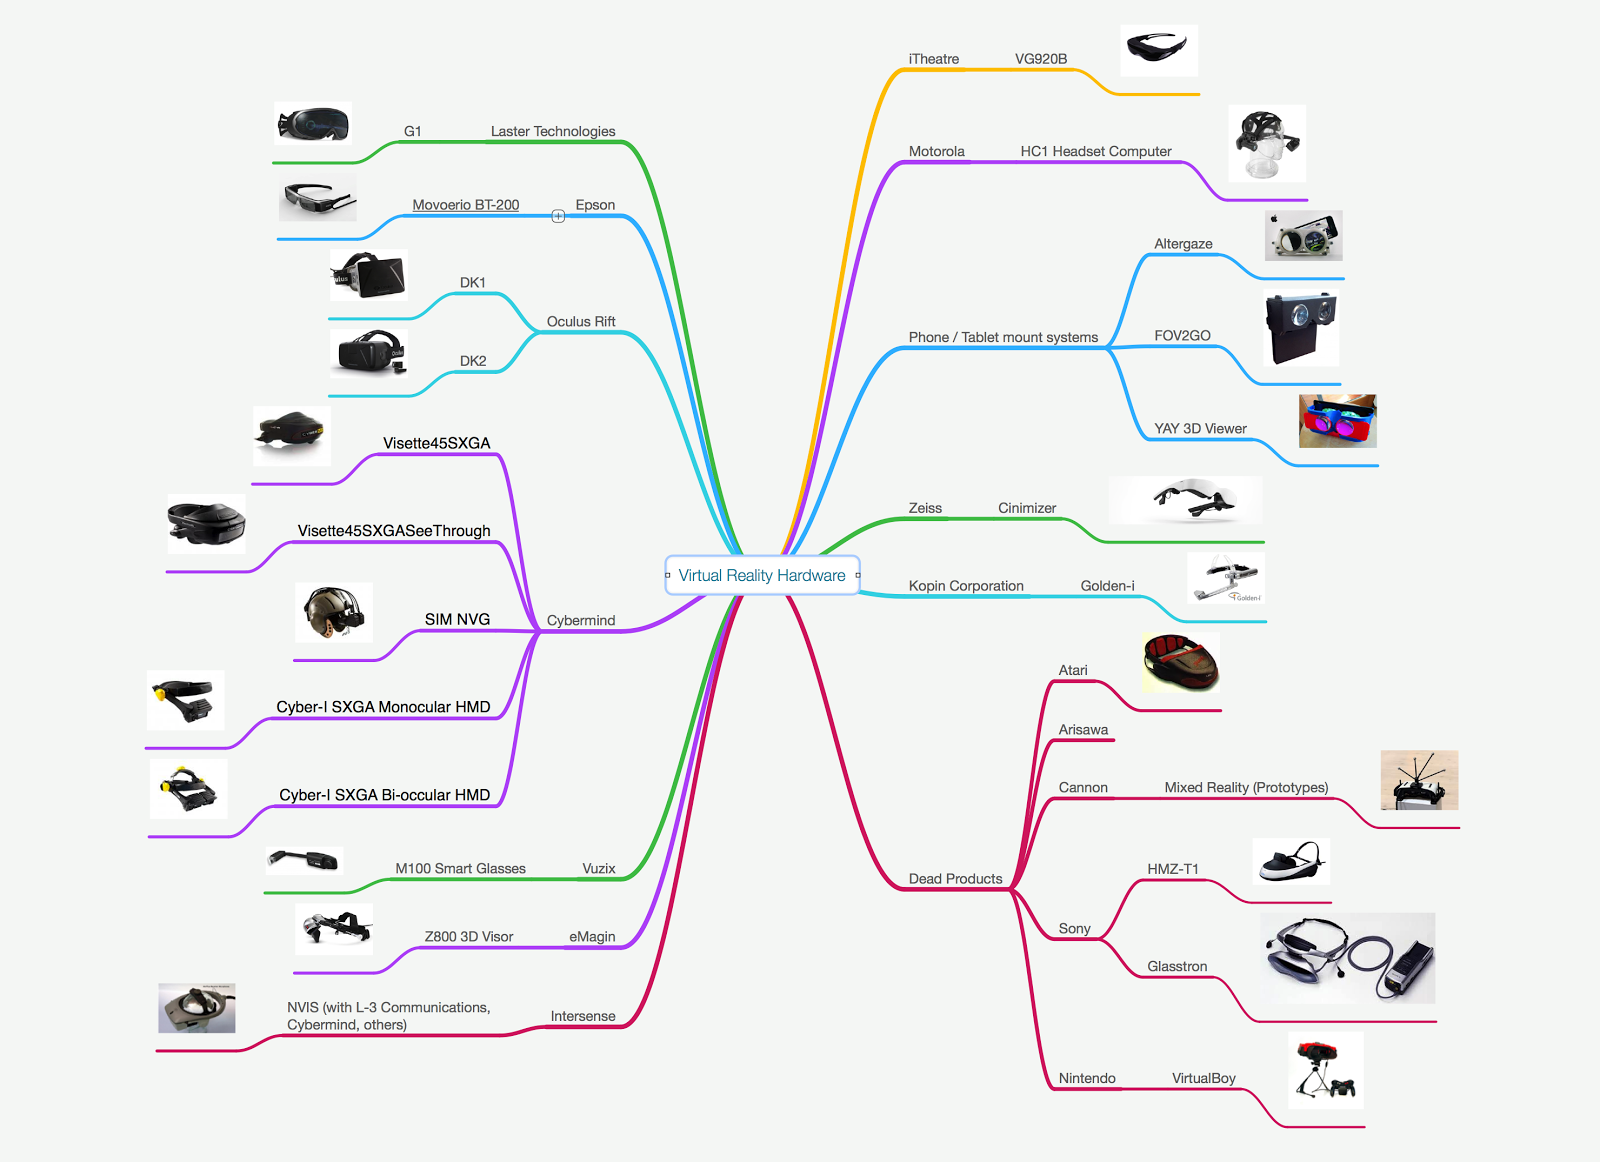
\includegraphics[width=0.8\textwidth]{resources/vr_headsets}
    \caption{AR and VR Products (an incomplete set)}
    \label{fig:vr_headsets}
\end{figure}

The OculusRift DK1 was found to offer the highest performance at the lowest cost. The DK1 is also a suitable system due to the active development of the SDK, and large open source community surrounding the project. Future development of the SDK and the forthcoming release of the compatible DK2 should enable the project to be forward compatible with future hardware, if that is required.
\section{Related Projects}
There is no other known project using an Oculus Rift for the visualisation of connectome data. There have been a small number of projects on using Virtual Reality for connectome visualisation. 

The most similar known projects are:
\begin{itemize}
  \item \textbf{The Dynamic Connectome}, part of the CEEDS project: real time, visualisation of neural activity \cite{ceeds2014}.
  \item \textbf{The Glass Brain Project}: real time, visualisation of neural activity \cite{GlassBrain2014}.
  \item Project work at Aachen University \cite{Rick2011}: using MOCAP and a CAVE virtual environment to interactively view a connectome with dynamic clipping \cite{ceeds2014}.
  \item Project work at Purdue University \cite{Chen2011}: using a CAVE virtual environment to view a connectome.
  \item \textbf{Brainder} \cite{brainder2014}, Dr Anderson Winkler’s excellent blog on FMRI and Blender rendering.
\end{itemize}


The Glass Brain Project uses a Unity 3D model of the brain, though it subsequently renders a 2D image from the model for display on LCD monitors. As such it does not obtain many of the benefits of the 3D model, nor have to face the challenges of displaying images in 3D.

The Dynamic Connectome project and the Aachen University and Purdue University projects use computer assisted virtual environment (CAVE) virtual reality rooms with multiple projectors rather than a head mounted display (HMD) system as proposed here. Such a system removes the requirement to wear bulky headgear, but instead requires a multi-projector system and dedicated room of projection screens. In addition to these requirements, the CAVE systems do not typically show 3D, nor do they update the view based on the user’s precise head position.

The Brainder project uses the open source ‘Blender’ 3D modeling software to ray trace brain models, primarily for use as 2D illustrations. Although the goals of Brainder are different from this project, the existence of (relatively) simple 3D brain models may be a useful asset. 



\section{Introducing the Rift DK1}
\section{Collimating Optics and Software Compensation}
\section{Integrated Sensors and the HMD}

\chapter{Extending VTK}
At the end of Chapter 4, the VTK pipeline had been configured so that connectome data could be loaded, manipulated using interactors, and rendered as a stereo-pair. Chapter 5 then noted that the collimating lenses in the Rift would distort any images sent to the rift. This chapter describes how image processing in software can be used to compensate for optical artefacts, and how GLSL shaders can be used with VTK in order to apply the image correction in real time. 

\section{The Need for Shaders}
\label{sec:need_for_shaders}
Why use shaders?
Discuss the problems of correcting optical artefacts using optics.
Discuss the problems of correcting optical artefacts using CPU. 
Discuss the suitability of using shaders to do these calculations!

\section{Applying GLSL Shaders to Materials}
One drawback of large open source projects is that the most widely available documentation for the project can quickly become outdated. In this regard, VTK is a victim of it's own success. When setting out to integrate GLSL shaders with VTK a lot of the documentation suggests that the shader can be encapsulated within an XML file and then applied to an object as a material. This is also the approach suggested by some of the official documentation, where "To Do" and "In progress" comments create the deceptive appearance that these features are cutting edge. \textbf{Do not be fooled!} This use of shaders is deprecated, and has not been possible in 'recent' VTK versions for most of the last decade. Due to the size of the project it can be difficult to find documentation for every feature of interest\footnote{If there is one thing harder than finding a needle in a haystack, it is finding a needle in a haystack where the needle was removed in 2006.}. 
Applying GLSL Shaders to VTK scenes via material properties is not feasible in current versions of VTK.

%http://www.vtk.org/Wiki/Shader_In_VTK

\section{Applying GLSL Shaders to Objects}
Having learned to ignore shader documentation pre-dating 2008, it transpired that shaders can be applied directly to VTK objects. This option approach contains  significant flaws. 

Firstly, if the fragment shader operates per material then it must be added to every material in the scene. This is not, by itself, a significant problem though it does mean that backgrounds cannot be distorted. Figure~TODO shows the effect of a simple fragment shader applied to a cone primitive. The shader is set to modify the colour of any cone fragment, with the result that all of the visible cone surface is modified.

Secondly, and more seriously, applying shaders per-object means that deformations are applied relative to the object's coordinates relative to it's renderer. The Rift, however, requires that the deformation to every screen pixel is applied as a function of that pixel's position on screen. VTK allows renderers to be placed within 'viewports' (TODO: need an image describing what a 'viewport' is...) in a renderwindow, and when the individual renderers are rendered each renderer only knows about its own relative size. The render window conceals information about the overall window size and location. (TODO: double check this). This problem could be addressed by using a different shader for each renderer.


\section{Applying GLSL Shaders to Buffers}
In order to achieve the desired shader deformation, two different approaches need to be combined. Default rendering passes need to be defined explicitly and combined into a Sequence Pass, and then a new rendering pass needs to be derived to perform the desire deformation to the entire render scene at once. The full system is represented in Figure~\ref{fig:vtk_extended_pipeline}.

\begin{figure}[htbp!]
    \centering
    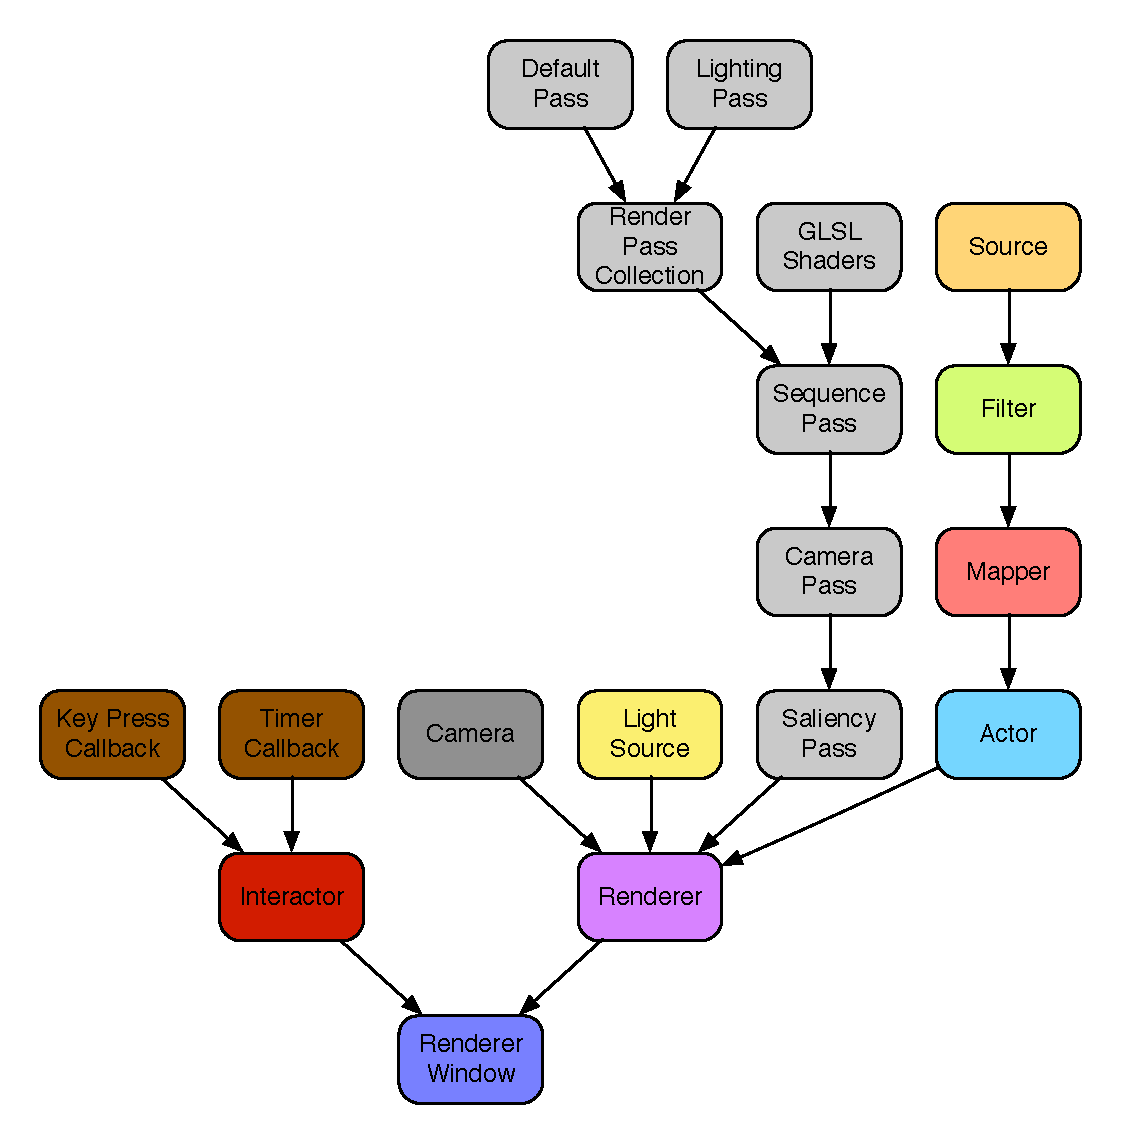
\includegraphics[width=1\textwidth]{resources/vtk_extended_pipeline}
    \caption{The Extended VTK Pipeline}
    \label{fig:vtk_extended_pipeline}
\end{figure}

Specifying the default rendering passes is necessary as VTK stops automatically defining them once the user manually configure any aspect of rendering. As shown in Figure~\ref{fig:vtk_extended_pipeline}, the default pass initializes the colour and depth buffers of the scene and the lighting pass sets up the scene lighting. VTK needs to apply these passes sequentially, and so they are grouped as a collection and then packaged into a Sequence Pass. The camera pass is applied after that sequence, and then the custom-made Saliency pass is applied. This is the point at which things start to get interesting.

The Saliency pass is derived from previous work by Dr Bernhard Kainz, and uses raw OpenGL code to perform off-screen rendering to a texture. This process, in effect, means that the scene is rendered to an area of memory on the graphics card instead of to pixels on the screen. The texture memory can be accessed very quickly by OpenGL functions, and is perfectly positioned for subsequent GLSL renderers.

\begin{figure}[htbp!]
    \centering
    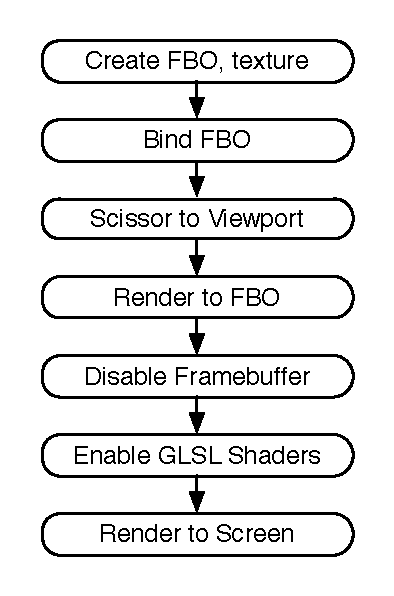
\includegraphics[width=0.4\textwidth]{resources/vtk_saliency}
    \caption{The New VTK Saliency Pass}
    \label{fig:vtk_saliency}
\end{figure}

TODO: This high-level description neatly side-steps the various issues of loading shaders, upgrading from glARB classes to modern glCore functions, ensuring that GLSL 440 was supported, upgrading the drivers, and the operating system, in order to get sufficiently recent NVIDIA support, and then dealing with the OpenGL bugs that recent versions of the NVIDIA drivers contain!! Though none of that was 'news-worthy', it took a great deal of time and patience to identify and fix. 

\section{The Shaders Themselves}
GLSL shaders are (ab)used to perform three functions in this project. They shift the image in order to align the camera viewpoint centre with the lens centre. They apply a pincushion deformation of the entire image in order to compensate for the barrel deformation of the Rift's lenses.  They also mask the edges of the screen where the OpenGL 340.x drivers leave image artefacts. 

It is assumed that the reader is familiar with the nature of shaders, and so the discussion here will not introduce the concept but rather will focus on the unusual way in which they are being employed. 

Figure~\ref{fig:rift_screen} shows how the lens positions, aligned with the user's eyes, are not aligned with the centre of the screen. This presents a problem, as the VTK cameras produce a viepoint that does not align with the user's eyes. The fragment shader code is executed for every pixel in the screen. Focussing first on the left-eye image, every fragment shader position is laterally offset by the lens centre to screen centre displacement. For the rift DK1 this involves a y-adjustment of 48 pixels. So when the shader is called for a pixel at (0, 0) the offset is applied and all subsequent calculations are made for a pixel at (48, 0). This is somewhat of a brute force solution, and will require revision for new hardware with different screen offsets. But given the hardware differences between the DK1 and DK2, it is likely that the shader code would need to be completely re-written.

\begin{figure}[htbp!]
    \centering
    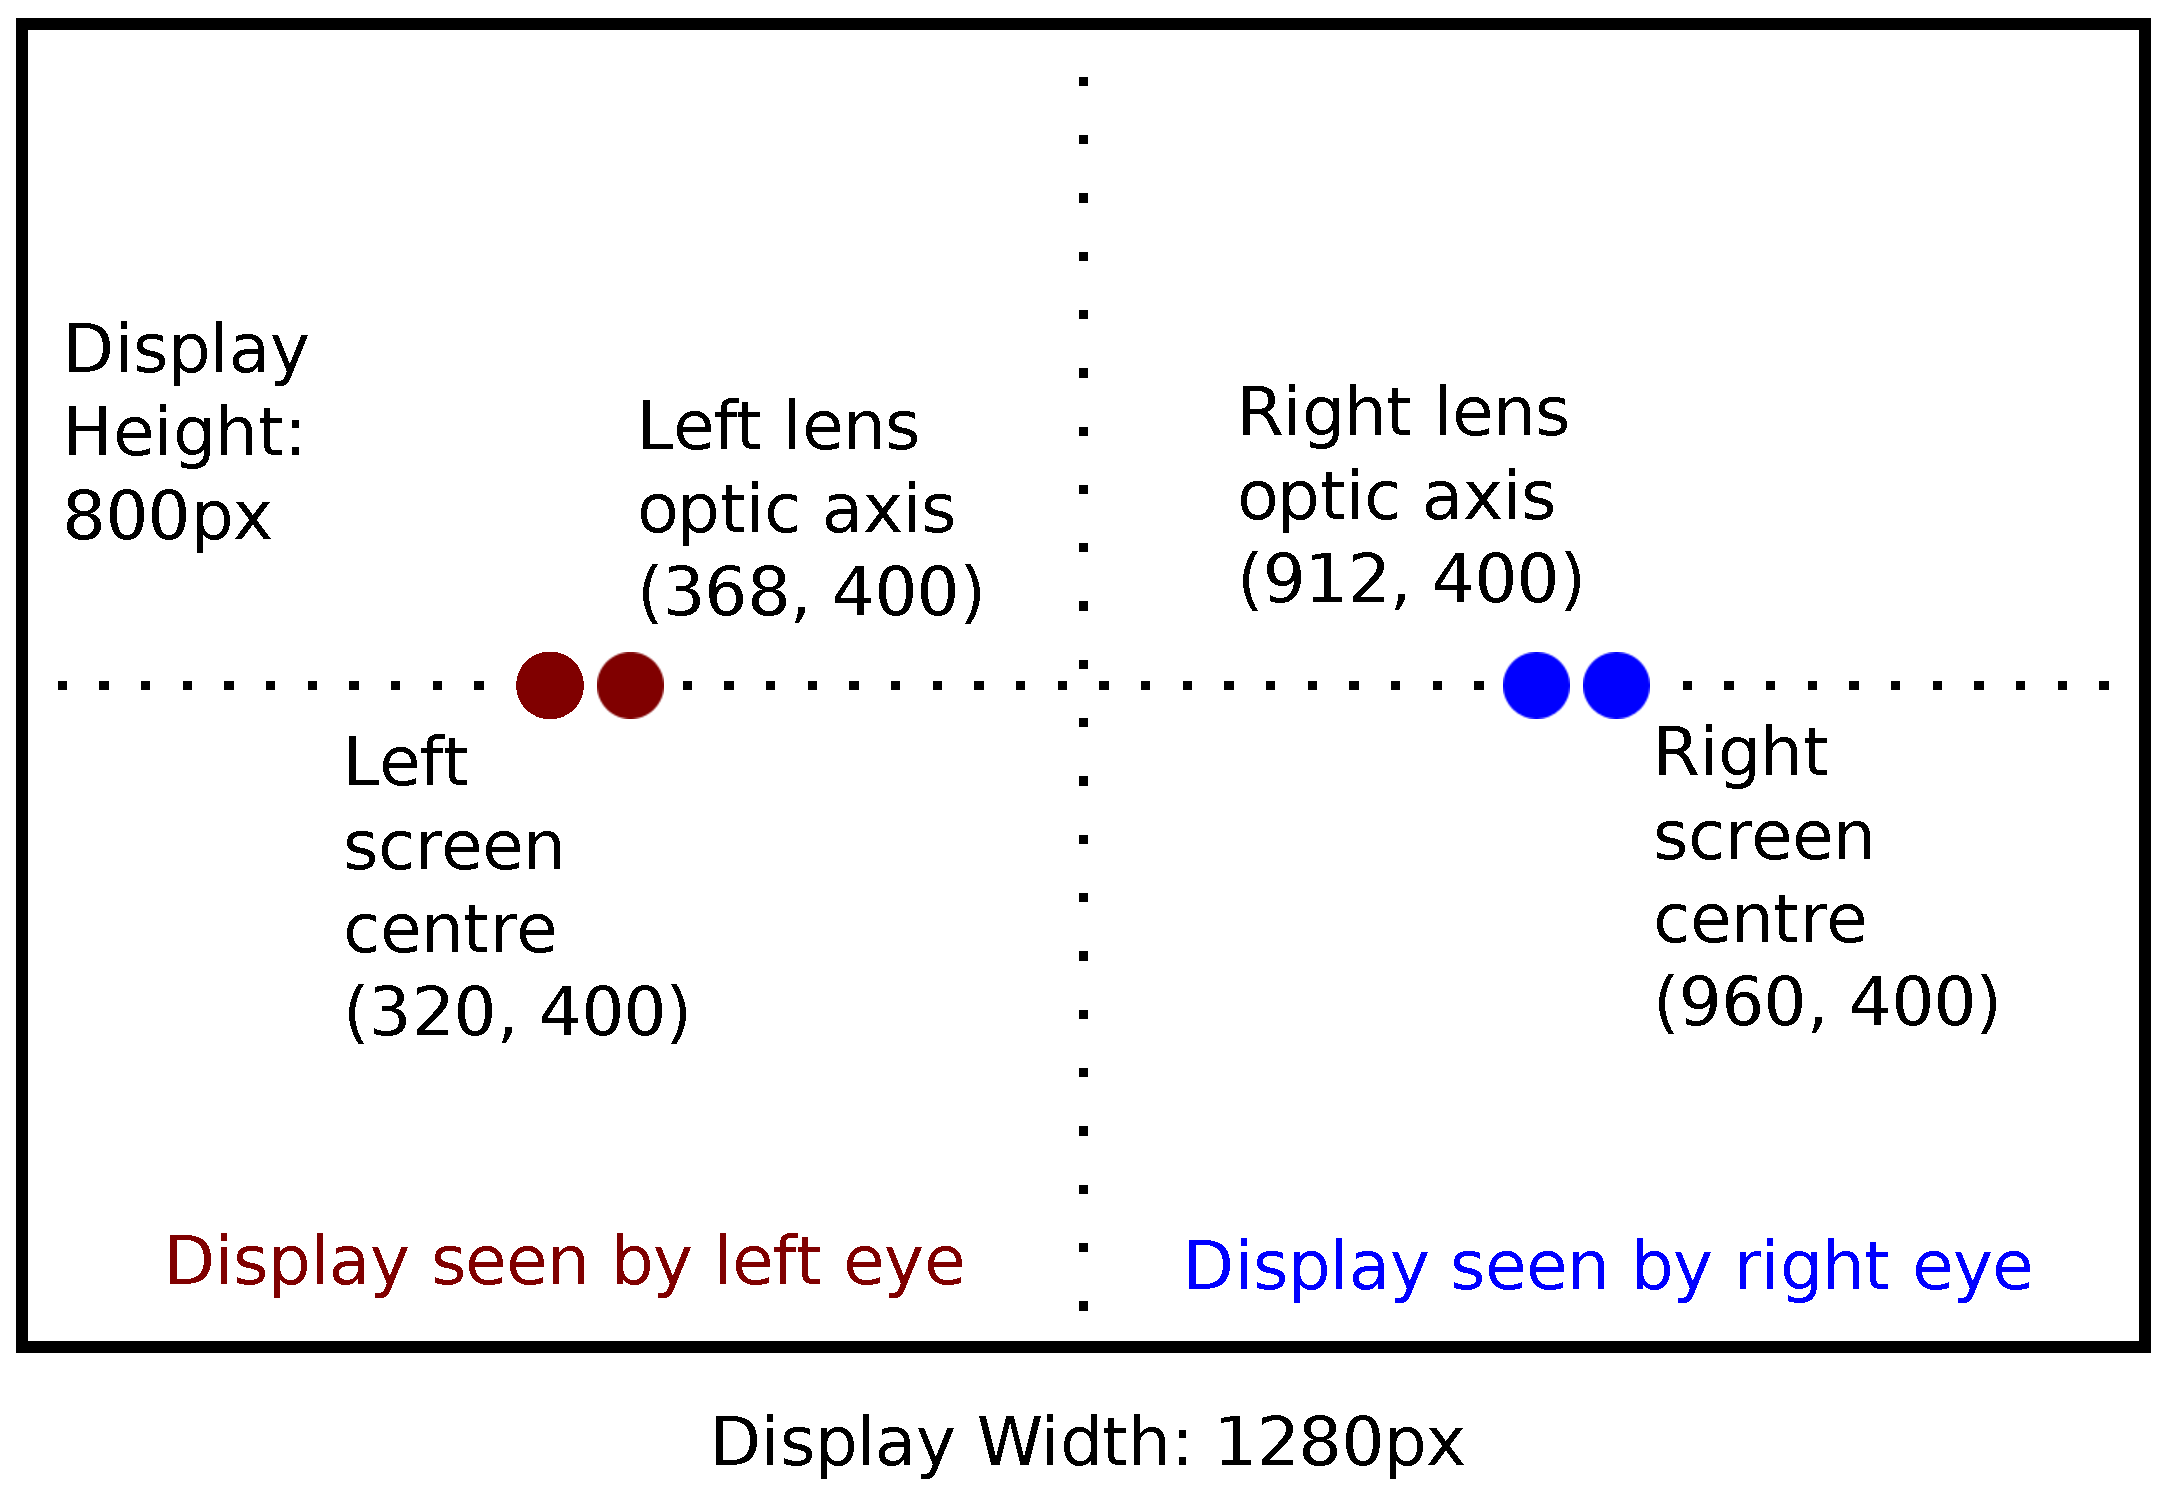
\includegraphics[width=0.8\textwidth]{resources/rift_screen}
    \caption{Lens and Screen Centres on the Rift Display}
    \label{fig:rift_screen}
\end{figure}

After correcting for the lens centre displacement, the shader then needs to pre-emptively correct for the barrel distortion of the Rift lenses. This is achieved using a polynomial function of the pixel's radial displacement from the lens centre. The polynomial function is based on reverse engineering of the Rift SDK TODO: cite shader forum, and with parameters obtained from Dr Stephan Rogge TODO: another citation. 

TODO: Ask Daniel if there should be some maths in here. It all seems a little bland!

\begin{figure}[htbp!]
    \centering
    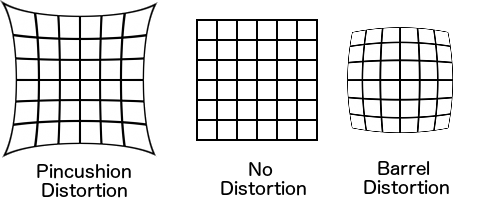
\includegraphics[width=0.8\textwidth]{resources/distortions}
    \caption{Distortions Applied to a Reference Grid}
    \label{fig:distortions}
\end{figure}

After correcting for the lens distortion, it is desirable to apply a chromatic aberration factor in order to mitigate the dispersive effect of the Rift's lenses as mentioned in Section~\ref{sec:need_for_shaders}. The parameters for the chromatic aberration correction were not available, and so approximate parameters were chosen based on empirical testing. TODO: give this a go. 

\section{Practical notes}
I *want* to complain here about how frustrating some of the driver problems were. Particularly the bug in NVIDIA 331.32 that "could prevent OpenGL Framebuffer Objects (FBOs) from being properly redrawn after a modeswitch.". Yes, NVIDIA, that bug certainly could! It took a long time to confirm that the problem was not due to my FBO rendering process, but rather due to driver problems.


\section{Other Approaches}
In theory, the Rift SDK can apply deformations directly, and since v0.3 Oculus have stated the SDK-rendering is the preferred approach. All of the example code for SDK-rendering was for a Windows system with DirectX rather than OpenGL, and it was decided that directly using GLSL shaders would be a more feasible approach given the project time frame. 

\chapter{Results}
\section{Automated Testing with CTest}
\section{Hardware Limitations}
\section{Software Limitations}
\section{Human Factors}


\chapter{Conclusion}
\nocite{Margulies2013}

\bibliography{bibtex/connectome}	
\bibliographystyle{unsrt} % unsrt == order of appearance, != alphabetical


\end{document}